\setchapterstyle{kao}
\setchapterpreamble[u]{\margintoc}
\chapter{Keeping track of time: Accuracy and precision in Real Time Clocks}
\labch{time_keeping}

For taking sensor readings to measure environmental conditions, and for many other uses of microcontrollers, it’s often important to have a reliable measure of time. 
In some cases, the sensor data are themselves based on elapsed time.
For example, wind speed is often calculated from the time elapsed during rotations of the propeller on an anemometer. 
The period of ocean waves may be calculated from the elapsed time between peaks and troughs. 
More generally, even if a sensor reading does not depend directly on elapsed time, it is likely to be far more useful if it is combined with a timestamp recording when it was taken. 
This places it in the context of previous and subsequent readings, concurrent readings by other sensors, position within the track of a moving ship, and so on.


In this chapter, you will set up and assess three ways of determining time with your \texttt{ESP8266}:
\begin{enumerate}
	\item Using the on-board \texttt{Real Time Clock} (often abbreviated as \rtc). 
	Like most modern microcontrollers, the ESP8266 has a built-in \rtc, which a measurement of the current time available through MicroPython. 
	These are very convenient to use, but vary widely in their reliability.

	\item Using an \rtc mounted on an external circuit board, called a \DS3231, that communicates with your microcontroller via a digital protocol called \i2c.

	\item From the Internet, using a utility called \texttt{Network Time Protocol} (\ntp). 
	This utility is the way your desktop and laptop update their internal clocks to maintain accuracy. 
	Your microcontroller can do the same thing!
\end{enumerate}
Each of these time-keeping methods has an important role to play in environmental sensing. 
We will explore the advantages and disadvantages of each method partly in this chapter, and in more depth during construction and deployment of field instruments for environmental monitoring in \refch{instr_constr}.

\begin{table}[h]
	\caption[\refch{time_keeping} materials]{\textbf{Materials you'll need\dots} 
		
		See Table \ref{tab:materials} for additional information.}
	\labtab{materials_time_keeping}
	\begin{center}
		\raggedright
		%\begin{tabular}{ c c c c } 
		\begin{tabular}{ c r c}
			\hline
			Sections & item & link \\
			\hline
			\multirow{2}{4em}{\refsec{set_read_time}} 
			& breadboard & \ref{mat:bb} \\
			& ESP8266 ``Feather'' & \ref{mat:mc} \\
			& micro-USB cable & \ref{mat:usb_cbl} \\
			%		\hline
			%		\multirow{3}{4em}{\vrefsec{circuits}}  
			& male-male jumpers & \ref{mat:jmp_mm} \\ 
			& pliers & \ref{mat:plr} \\ 
			& DS3231 RTC & \ref{mat:RTC} \\ 
			\hline
		\end{tabular}
		
\end{center}\end{table}

\section{Accuracy and precision}
\labsec{acc_prec}
A key idea in this chapter is that no time-keeping device is perfect. 
All have at least \textit{some} errors. 
To choose the best method of keeping time, and to know how far off our references to time are likely to be, we need metrics to measure the errors associated with each method. 

The most important metrics for quantifying errors in time-keeping %(as well as in other sensors) 
are  \textbf{accuracy} and \textbf{precision}. 
In everyday language, we might use these terms more or less interchangeably.
In science, however, they have quite different meanings:

``Accuracy'' refers to a systematic \emph{bias} in measurements.
For example, we say a clock runs ``fast'' if it consistently reports more time having passed than the true time.
The clock runs ``slow'' if it consistently reports less time having passed than the true time.
Both of these errors reflect lack of accuracy -- this clock is, on average, \emph{biased} towards under- or over-estimating the true passage of time.

Under some circumstances, we might be able to increase accuracy with a \textbf{calibration}.
A calibration is a quantitative relationship between a measurement and a true physical parameter (in this case, time).

For example, if we know a clock runs fast by two minutes per day, we might calibrate that clock by calculating the ratio of the number of seconds in a day (60 seconds per hour $\times$ 60 minutes per hour $\times$ 24 hours per day) to the number of seconds reported by the clock (60 seconds per hour $\times$ 60 minutes per hour $\times$ 24 hours per day + 2 $\times$ 60):
\[ 
\frac{60 \times 60 \times 24}{60 \times 60 \times 24 + 2 \times 60 } = \frac{86400}{86520} = 0.99861
 \]
This calibration tells us that if we multiply the clock's measure of elapsed time by the factor 0.99861, we compensate for its biased tendency to run fast.
This adjusted time will be much more accurate than the clock's nominal time reading.

``Precision'' refers to the \emph{scatter} in a large number measurements of the same physical quantity. 
For example, if we use a stopwatch to repeatedly time an event that we know to take exactly one hour, one measurement might be 3595 seconds, the next might be 3605 seconds, and so on. 
These deviations among measurements (in this case, a difference of 10 seconds between successive measurements) represent lack of precision. 

Because these errors are random, or at least unpredictable, we cannot devise a calibration to mitigate them. 
However, under some circumstances, we might be able to take an average or median of many measurements. 
If so, the precision of this average or median is often much better than the precision of a single measurement.

It's important to recognize that accuracy and precision reflect distinct characteristics of a dataset. 
A set of measurements can be accurate but not precise, precise but not accurate, both precise and accurate, or both inaccurate and imprecise. 


\section{Setting and reading time on the ESP8266}
\labsec{set_read_time}
The exercises in this chapter have two parts. 
In this, the first part, you will set up and test the hardware and software needed to use the three methods of time-keeping. 
In the second part, you will assess the relative accuracy and precision of the on-board and external RTCs, relative to NTP (Internet) based time-keeping.

\subsection{The On-Board RTC}
Your ESP8266 microcontroller arrives from the factory with a clock already built into it and accessible through MicroPython codes. 
We will refer to this clock as the \emph{on-board RTC}, to distinguish it from other sources of time like external devices or the Internet.
Because the on-board RTC is already present on your microcontroller, it can be accessed without any additional hardware --- we need only execute a few Python commands. 

\subsubsection{\howto Read and set the on-board RTC}
To use the on-board RTC:
\begin{enumerate}
	\item \textbf{Import the \rtc method from the machine module and create an instance of the RTC class}:
	\begin{lstlisting}[language=Python]
	from machine import RTC
	rtc = RTC() 
	\end{lstlisting}
	Here, \lstinline{rtc} is the variable name for an instance of the \rtc object.
	\item \textbf{Query} \lstinline{rtc} \textbf{to obtain a time reading from the on-board \rtc}:
	\begin{lstlisting}[language=Python]
	rtc.datetime() # get date and time
	\end{lstlisting}
	The format of the output from this command is a Python \htmladdnormallink{tuple}{https://docs.python.org/3.3/tutorial/datastructures.html\#tuples-and-sequences}: \texttt{(year, month, day, weekday, hour, minute, second, microsecond)}.
	
	Note that the on-board \rtc initially has a default time that has no bearing on the actual time.
	\sidenote[][*-22]{\begin{kaobox}[backgroundcolor=\SNcolor,frametitlebackgroundcolor=\SNcolor,frametitle=Wrinkles in time\dots]The onboard \rtc is turned off whenever the power is shut off to the ESP8266. That means if you unplug your ESP8266 from the USB cable (and if there is no battery to keep it powered up) the on-board \rtc will be reset to its default time.
	You must then reset it to have the correct time.
	However, if you reboot the microcontroller while keeping power on, the onboard \rtc stays on and preserves the current time. The onboard \rtc also preserves the current time when it goes into ``deepsleep'' to save energy.\end{kaobox}} 
	  
	\item \textbf{Set the current time on the on-board RTC with the command}
	\begin{lstlisting}[language=Python]
	rtc.datetime((2017, 8, 23, 1, 12, 48, 0, 0)) # set a specific date and time
	\end{lstlisting}
	In this example, the year is 2017, month is August (the 8th month), day is 23, weekday is 1, hour is 12, minute is 48, second is 0, and microsecond is 0. Try it (ideally with a more nearly correct time!) and check to make sure the time has been reset according to your command.
\end{enumerate}

Further information about using the on-board RTC can be found at Micropython.org's \htmladdnormallink{Quick Reference}{
http://docs.micropython.org/en/latest/esp8266/esp8266/quickref.html} and
\htmladdnormallink{Code Library}{http://docs.micropython.org/en/latest/esp8266/library/machine.RTC.html} documentation.

\subsection{Network Time Protocol (NTP)}
As you likely noticed in the previous step, it is difficult to set the on-board RTC from the command line with high accuracy. 
A more convenient and accurate way to set the clock is to use an online time source.
A human-readable example is the \htmladdnormallink{official time source}{https://www.time.gov/} for the U.S. government, operated by the National Institute of Standards and Technology (NIST).

For computers and microcontrollers, online time sources are easier to use with a machine-readable format called  
 \texttt{Network Time Protocol}, or \texttt{NTP}. 
An \texttt{NTP} server is an online portal using this protocol that enables a local machine to calculate the current time.  
Micropython has a built-in utility called \lstinline{ntptime} to automatically obtain the current time from an NTP server (the default is \texttt{pool.ntp.org}), if it is connected to the Internet via WiFi. 
\lstinline{ntptime} can also reset the on-board \rtc, to match the time from the NTP server. \todo{Create a box or hyperlink to the explanation of how NTP works.}
%We’ve provided a modified version of this utility, which can also be used in the next step to reset the external RTC.

%\marginnote{NOTE: 
	This part of the exercise assumes that your ESP8266 is connected via WiFi in \texttt{Station mode} to the Internet. If it is not, follow the instructions in \refsec{wifi_sta} to establish this WiFi connection, then continue with the exercise.
%} 

\subsubsection{\howto Obtain current time from the Internet}
To use an online NTP server to set the on-board \rtc to the current time:
\begin{enumerate}
	\item \textbf{Use} \lstinline{ntptime} \textbf{to get the current time from the NTP server with the commands}:
\begin{lstlisting}[language=Python]
import ntptime, utime
t=ntptime.time()
print('The result of ntptime.time() is: ',t)
print("Converted to human-readable time that's: ",utime.localtime(t))
\end{lstlisting}
	Note that the results of \lstinline{}
	\item \textbf{Set the time on the \texttt{ESP8266}’s internal RTC}:
\begin{lstlisting}[language=Python]
ntptime.settime()
\end{lstlisting}
	This command automatically retrieves the current time from the NTP server, and uses it to set time on the on-board RTC.
	\item \textbf{Query the on-board \rtc to verify the correct time has been set}:
\begin{lstlisting}[language=Python]
rtc.datetime() # get date and time
\end{lstlisting}
	You should see that the time has been set quite accurately to \texttt{Coordinated Universal Time} (\texttt{UTC}). 
\end{enumerate}


\subsection{DS3231 (external) RTC}
Our third method of keeping time is using an external RTC, known as a \DS3231.
The \DS3231 is an \rtc similar the ESP8266's \rtc, but with two important differences. 
One is that the \DS3231 has a coin cell battery.
This means that it keeps track of time, even when the microcontroller to which it's attached is powered down.
The other is that the \DS3231 is a specialized device, that performs only time-related functions. 
In \refsec{rel_acc}, we'll assess the accuracy and precision of this specialized time-keeping device compared to the ESP8266's onboard \rtc.

The \DS3231 interacts with a microcontroller using a \texttt{digital} protocol known as \i2c. 
The \i2c protocol is discussed in detail in \refch{telem_sens_coms}.
For now, the attribute of the \i2c interface we're most interested in is that it's very easy to set up. 
Connecting the \DS3231 external \rtc to your microcontroller requires just a few jumpers. 


\subsubsection{\howto Set up an external \rtc}




As you set up your circuit, refer to the example layout in \reffig{ds3231_breadboard}. 
Because there is only one component in this exercise, you have a lot of flexibility where to place your components and jumpers.
\begin{marginfigure}
	\begin{center}
		\htmladdnormallink{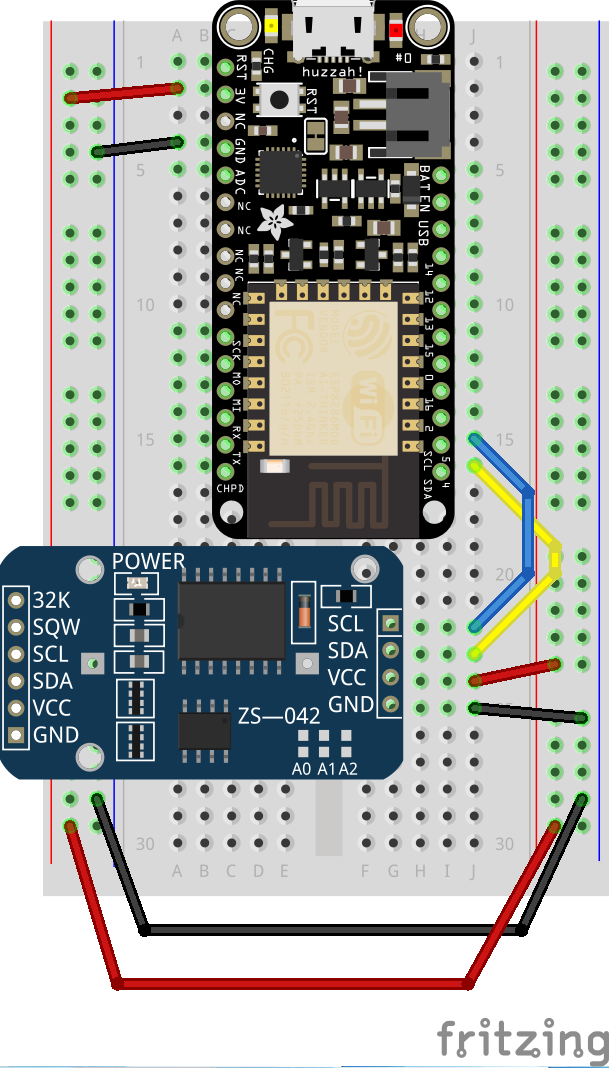
\includegraphics[width=\MFW]{Fritzing/feather_DS3231.png}}{https://publicsensors.org/IntroSensors/Fritzing/feather_DS3231.png}
		%\includegraphics[height=5cm]{Images/DS3231breadboard.jpg}
		\caption[DS3231 on breadboard]{An example of layout and wire connections for the DS3231 external Real Time Clock and ESP8266 microcontroller.}
		\labfig{ds3231_breadboard}
	\end{center}
\end{marginfigure}
\begin{enumerate}
	\item \textbf{Insert the coin cell battery into the battery holder (if it is not already in) with the positive (+) side out.}
	\item \textbf{Connect the GND and 3V pins on the ESP8266 to the GND and Vcc pins on the DS3231}. 
	
	You can do that directly with long jumpers, or (more neatly) using the positive and negative rails with short jumpers as in \reffig{ds3231_breadboard}.
	\item Connect the \texttt{SDA} (\#4) pin on the ESP8266 to the \texttt{SDA} pin on the \DS3231, and the  \texttt{SCL} (\#5) pin on the ESP8266 to \texttt{SCL} on the \DS3231.
	\item \textbf{Download the driver module provided by Adafruit called \htmladdnormallink{urtc.py}{https://github.com/adafruit/Adafruit-uRTC} for the \DS3231 \rtc.}
	
	Save it into a \texttt{Codes} directory on your computer.
	
	\item \textbf{Copy } \lstinline{urtc.py} \textbf{onto our microcontroller, using either the \texttt{WebREPL} or \mpfshell methods from \refch{connect}.}  
	\item %You are now ready to test your \DS3231 \rtc. 
	\textbf{Set up the \i2c connection to your \DS3231:}
\begin{lstlisting}[language=Python]
import urtc
from machine import I2C, Pin
i2c=I2C(scl=Pin(5),sda=Pin(4))
rtc3231=urtc.DS3231(i2c)
\end{lstlisting}
	\item Query the time from your \DS3231, with:
\begin{lstlisting}[language=Python]
rtc3231.datetime()  # print out current date/time tuple
datetime = rtc3231.datetime() 
print(datetime.year)          # Or, print out separate elements
print(datetime.month)         # of the date/time tuple
print(datetime.day)
print(datetime.weekday)
print(datetime.hour)
print(datetime.second)
\end{lstlisting}
\end{enumerate}

To set the time on the \DS3231 using the \ntp server, the easiest method is to use the following utility, called \texttt{SetTimeDS3231.py}:
\lstinputlisting[language=Python,label=SetTimeDS3231,caption={\htmladdnormallink{\texttt{SetTimeDS3231.py}}{https://publicsensors.org/IntroSensors/Codes/SetTimeDS3231.py}: A Micropython utility to set a \DS3231 \rtc to time from a Network Time Protocol (NTP) server.}]{Codes/SetTimeDS3231.py}
%\lstinputlisting[language=Python]{Codes/settimeDS3231.py}
\begin{enumerate}[resume]
	\item \textbf{Download} \lstinline{SetTimeDS3231.py}\textbf{, copy it onto your microcontroller, and execute:} 
\begin{lstlisting}[language=Python]
from SetTimeDS3231 import settimeDS3231
datetime = rtc3231.datetime()  # obtain and print the pre-existing time
print(datetime)                
settimeDS3231()                # set the DS3231 with NTP
datetime = rtc3231.datetime()  # obtain and print the
print(datetime)                # NTP-set time
\end{lstlisting}
	Try it and confirm that the time on the \DS3231 \rtc has been set correctly. 	
\end{enumerate}

You can also set your on-board \rtc from the \DS3231 by pasting (with \texttt{<ctrl>-e}/\texttt{<ctrl>-d} and executing the following two lines:
\begin{lstlisting}[language=Python]
tDS3231=rtc3231.datetime()
rtc.datetime((tDS3231.year,tDS3231.month,tDS3231.day,0,tDS3231.hour,tDS3231.minute,tDS3231.second,0))
\end{lstlisting}

More information about the \DS3231 \rtc can be found at \htmladdnormallink{http://micropython-urtc.readthedocs.io/en/latest/}{http://micropython-urtc.readthedocs.io/en/latest/}.

\loadMilestone{mlst:03} % load milestone with tags id: mlst:02


\section{Accuracy and precision of time-keeping on the ESP8266}
\labsec{rel_acc}
Now that your ESP8266 is set up to use all three methods to obtain the current time, we can consider how to use them most effectively for environmental sensing. 

Some considerations involve practical constraints. 
For example, in many field deployments of environmental sensors WiFi is either unavailable or available only intermittently, such as when a cell phone is used to create a temporary hotspot.
This constrains when \ntp is a viable option.
To save battery power, a microcontroller in an environmental sensor often puts itself to ``sleep'', waking up only briefly at preset intervals to take measurements.  
This wake-up function usually operates through the on-board \rtc, so this device must be used in at least some aspects of time-keeping. 

Other considerations involve the \emph{quality} of the temporal data from each of the three sources. % --- that is, their accuracy and precision. 
Because no time-keeping device is perfect, we expect that measurements of time intervals using any of these methods will result in a distribution of measured values, with varying deviations from the true values. 
The deviation of the center of this distribution from the true time corresponds to an \emph{accuracy} metric. 
The breadth of the distribution corresponds to a \emph{precision} metric. 
Together, accuracy and precision metrics enable us to anticipate how errors in time-keeping might accumulate during the deployment of an environmental sensor.

To decide how best to select among time-keeping methods for environmental sensing, we need to answer questions like: 
\begin{itemize}
	\item How big are the time-keeping errors for each method (that is, how accurate and precise are each of the methods)?
	\item Are particular \rtcs biased towards run fast or slow (that is, are some units ``defective'' so that they differ \emph{systematically} from the overall population of \rtcs)?
	\item Does the magnitude or direction of timekeeping error depend on environmental conditions (for example, do higher or lower temperatures affect time-keeping accuracy and precision)?  
\end{itemize}

To answer these questions objectively, we need two things:
\begin{itemize}
	\item A \emph{dataset} of simultaneous time measurements by different methods, that quantifies errors as relative differences in estimated time between methods; and,
	\item \emph{Statistical analysis} that enables us to visualize the error distributions, establish bounds for likely time-keeping deviations, and test hypotheses about performance of individual devices.
\end{itemize}
In this section, we will go step-by-step through the process of generating a dataset and analyzing it, to make inferences about time-keeping accuracy and precision. 
In addition to helping us devise a good strategy for tracking time for field sampling, these steps will be good preparation for generating and analyzing datasets from environmental sensors you will build and deploy in later chapters.


\subsection{Generating a dataset of time-keeping errors}
In generating data to characterize time-keeping, a few simplifications can greatly reduce the required effort. 
One of those is to consider only relative deviations among the on-board and \DS3231 \rtcs, compared to time from an \ntp server. 
This makes sense because \ntp servers are in general very accurate, and because we don't have an easily accessible alternative time source that is more accurate.
So, in effect, we will regard \ntp as giving the ``correct'' time.

Another simplification is to take time-keeping error samples over relatively short periods. 
On a deployment, an instrument might spend weeks or months without access to \ntp or any other means of correcting errors. 
Observing \rtcs over comparably long periods would give the most realistic assessment of time-keeping errors.
However, this is almost never practical during instrument design, assembly and testing.
We will therefore attempt to learn as much as possible using much shorter sampling periods.

\begin{kaobox}[frametitle=A download-able dataset of time-keeping errors]
	In a classroom setting with multiple microcontrollers and \rtcs (ideally 10 or more), generating your own dataset with the steps outlined below is the most informative strategy. 
	If you do not have access to a sufficient number of devices, or if you would like to focus on understanding the data analysis rather than acquiring new data, you can download an \htmladdnormallink{archived dataset}{https://publicsensors.org/IntroSensors/Codes/TimeDataExamples.zip} of time-keeping errors.
	This archive ``unzips'' to provide a directory called \lstinline{TimeData} containing 90 
	time-keeping error data files.
	You can use these files instead of your own dataset.
	
	\smallskip
	Alternatively, you can collect data for your own devices and compare them to the archived data. 
	However, to use the archived data in this way, you must use parameters for your data collection that are consistent with those use to generate the archive: 
	
	\lstinline{interval_sec=10*60, n_samples=12, n_replicates = 4}
%	\begin{lstlisting}[language=Python]
%	interval_sec=10*60
%	n_samples=12
%	n_replicates = 4
%	\end{lstlisting}
	
	As explained below, this corresponds to four replicates, each with 2-hour sequences of sampling at 10 minute intervals.
\end{kaobox}

\subsubsection{\howto Generate a time-keeping dataset}
To make generating a dataset easy, we’ve provided a Micropython function that automatically sets the on-board and \DS3231 \rtcs so that they initially agree with \texttt{NTP} time.
The function then records a sequence of time samples from each, and saves them to a data file.
This process is repeated a specified number of times, each time producing a new data file, to produce a replicated dataset. 

Follow these steps to generate your dataset:
\begin{enumerate}
	\item \textbf{Connect your microcontroller to \texttt{WiFi} in \texttt{STA} mode, so it can access the \texttt{NTP} server.}
	\item \textbf{Download the file} \todo{Include several passes through NTP connection because it's not always successful even if internet is available.} \htmladdnormallink{TimeCompare.py}{https://publicsensors.org/IntroSensors/Codes/TimeCompare.py}\textbf{ onto your computer, and use }\lstinline{mpfshell} \textbf{or} \lstinline{WebREPL} \textbf{to copy it onto your microcontroller.}
	\item \textbf{Initialize the on-board and external (\DS3231) \rtcs:}
\begin{lstlisting}[language=Python]
from machine import RTC
import urtc
from machine import I2C, Pin
from TimeCompare import time_compare
rtc_ = RTC()  # Initialize on-board RTC
i2c = I2C(scl=Pin(5), sda=Pin(4))  # Initialize DS3231 (external) RTC
rtc3231_=urtc.DS3231(i2c)
\end{lstlisting}
	Note the ``\textunderscore'' in some of the variable names. 
	This is to distinguish them from similar variable names in the Micropython function.
	\item \textbf{Define the sampling parameters, a modification of:}
\begin{lstlisting}[language=Python]
prefix_='danny'        # Filenames will start with this
interval_sec=10        #  Sampling interval, in seconds
#interval_sec=1*60     #  A format making it easy to specify intervals in minutes
#interval_sec=1*60*60  #  A format making it easy to specify intervals in hours
n_samples= 10      # Number of time intervals to sample
n_replicates = 3   # Number of times to replicate the sampling protocol
\end{lstlisting}
	The meaning of these parameters is:
	\begin{itemize}
		\item[$\circ$] \lstinline{prefix} is used to generate informative names for data files.
		
		\smallskip
		In this case, filenames will have the form \lstinline{danny_dda01900_568621029.txt} (starting with the prefix, \lstinline{danny}). 
		The prefix is followed by the unique ID of the microcontroller (\lstinline{dda01900}), then a timestamp (\lstinline{568621029}) recording when sampling starts, and finally a suffix (\lstinline{txt}) indicating the file type.
		
		\smallskip
		This convention gives filenames that are informative --- because of the prefix and microcontroller ID, they can be identified easily by both humans and machines.
		Also, because the timestamp does not repeat itself, no file can be accidentally overwritten by another file with the same name. 
		\item[$\circ$] \lstinline{interval_sec} is the parameter determining the length of intervals (in seconds) at which time samples should be taken.
		
		\smallskip
		This example illustrates two ``tricks'' that many Micropython users find helpful when collecting and analyzing data.
		\begin{itemize}
			\item[$\triangleright$] When sampling at longer intervals (e.g. 3.5 hours) to explicitly write \lstinline{3.5*60*60}. 
			This expression is much easier to understand at a glance than the same number multiplied out (\lstinline{12600.0}). 
			\item[$\triangleright$] When exploring parameter space, to comment out rather than delete previous values. 
			This makes it far easier to keep track of what you've already tried.			
		\end{itemize}		
		\item[$\circ$] \lstinline{n_samples} and \lstinline{n_replicates} specify, respectively, how many samples each data file should contain, and how many data files should be created. 
		
		\smallskip
		The total duration of sampling for each file will then be \lstinline{interval_sec} $\times$ \lstinline{n_samples} seconds. 
		Sampling for all the replicates will last \lstinline{interval_sec} $\times$ \lstinline{n_samples} $\times$ \lstinline{n_replicates} seconds.
	\end{itemize}
	\item \textbf{Execute a short sampling run, with the command:}
\begin{lstlisting}[language=Python]
time_compare(prefix=prefix_,rtc=rtc_,rtc3231=rtc3231_,interval_seconds=interval_sec,num_samples=n_samples,num_replicates=n_replicates)
\end{lstlisting}
	
	It's a good idea to first do some short test sampling runs, with parameters set so that the entire process will take just a couple minutes.
	The parameters above are an example of this. 
	If there is a problem with hardware or WiFi, these parameters enable you to detect that quickly.
	
	\item \textbf{Inspect the on-screen output.}
	
	The \lstinline{time_compare} function has two types of output. It writes output to the terminal, which looks like this:
\begin{lstlisting}[language=Python]
****Beginning replicate  1  ****

Trying to set the DS3231 RTC using NTP...
setting urtc datetime to:  DateTimeTuple(year=2020, month=1, day=15, weekday=None, hour=2, minute=2, second=56, millisecond=None)
...successfully set from NTP

Creating data file:  danny_c9865800_632368922.txt

sample_num,day_onboard,hour_onboard,min_onboard,sec_onboard,day_external,hour_external,min_external,sec_external,day_NTP,hour_NTP,min_NTP,sec_NTP
0 15 2 2 56 15 2 2 56 15 2 2 56 
1 15 2 3 6 15 2 3 6 15 2 3 7 
2 15 2 3 16 15 2 3 16 15 2 3 17 
3 15 2 3 26 15 2 3 26 15 2 3 27 
4 15 2 3 37 15 2 3 37 15 2 3 37 
5 15 2 3 47 15 2 3 47 15 2 3 48 
6 15 2 3 57 15 2 3 57 15 2 3 58 
7 15 2 4 7 15 2 4 7 15 2 4 8 
8 15 2 4 18 15 2 4 18 15 2 4 18 
9 15 2 4 28 15 2 4 28 15 2 4 29 
10 15 2 4 38 15 2 4 38 15 2 4 39 
\end{lstlisting}
	The line of text above the array of data is a ``header'', explaining what the numbers in each column mean: 
	The first entry is a sample number.
	This is followed by day, hour, minute and second for the on-board \rtc, the \DS3231 \rtc, and the \ntp time server.
	
	\smallskip
	If the \ntp	\, server cannot be accessed, the last four entries are replaced by ``-1'', to make them easy to distinguish from real data:	
\begin{lstlisting}[language=Python]
sample_num,day_onboard,hour_onboard,min_onboard,sec_onboard,day_external,hour_external,min_external,sec_external,day_NTP,hour_NTP,min_NTP,sec_NTP
0 8 22 19 14 8 22 19 14 -1 -1 -1 -1 
1 8 22 19 41 8 22 19 41 -1 -1 -1 -1 
2 8 22 20 8 8 22 20 8 -1 -1 -1 -1 
\end{lstlisting}
	
	%	The top line in this output is a header, explaining what the numbers in each column mean.
	%	Each additional row is an observation of time readings from the onboard RTC, the DS3231 RTC, and (if your ESP8266 is online) the NTP server. 
	%	If your ESP8266 is not connected, it will record ``-1'' to make it easy to distinguish from real data.
	
	As you watch the output, it is easy to pick out differences in seconds, minutes etc. among the time stamps (if there are any).
	
	\item \textbf{Upload data files to your computer, and check that they are being written correctly.}
	
	Each line in the data files is the same as the data array printed to the terminal, except that there is no header line.
	
	\item \textbf{Agree with your classmates on a consensus set of sampling parameters.}
	
	The goal is to obtain a replicated set of time comparisons between time sources, across as many devices as possible. 
	To be comparable, all the data must be collected with the same sampling parameters.
	
	\smallskip
	In this discussion, keep in mind the tradeoffs among the total sampling time, the length of time over which deviations among time sources are tracked within each data file, and the number of data files for each microcontroller/\rtc combination. 
	
	\smallskip
	For example, if the class decides that a total of 8 hours of sampling time is a reasonable limit, then options include fewer, longer runs (e.g., 2 runs of 4 hours each) or more, shorter runs (4 runs of 2 hours each).
	Consider which parameter choices are most likely to provide a statistically informative dataset within the available time.
	
	\smallskip
	In designing this sampling scheme, it's important to be aware that the sampling can be started and stopped to accumulate more sampling runs.
	However, a sampling run is recorded into a data file only if it is allowed to complete.	For example:
\begin{itemize}
	\item[$\circ$] If you use the parameters \lstinline{interval_sec=6*60, n_samples=10, n_replicates=8}, this indicates a total sampling time of 8 hours (eight 3600 second sampling runs).
	
	\item[$\circ$] If you initially interrupt \lstinline{time_compare} after 3.5 hours, it will record the three data files for which sampling was completed, but will \underline{not} record data from the 0.5 hour run that was interrupted.
	
	\item[$\circ$] You can later restart \lstinline{time_compare} to run for another 5 hours, to collect the remaining replicates.
\end{itemize}	
	 
%	The files have informative names: they begin with the prefix (e.g. your name), followed by the unique ID of your microcontroller, followed by the timestamp at which they were created. 
%	This type of name, while it looks a bit clunky, has two key advantages: it makes sure that it is easy for both humans and machines to find the files they’re looking for (because the names all share name and ID); and, no files will be unintentionally overwritten (because each has a unique timestamp in its name). 
	
	
\end{enumerate}
\loadMilestone{mlst:03a} % load milestone with tags id: mlst:02


\subsection{Visualizing distributions of time-keeping errors}

With a set of data files from \lstinline{time_compare}, we can now assess whether, how much and in which direction our time sources deviate from each other. 
%By quantifying these deviations we will get a sense for the relative accuracy and precision of each method of determining time.
Until now, you have used Micropython on your microcontroller, to interact with devices and collect data.
In this section, you will work with Python \emph{on your computer} to open, parse and statistically analyze these data to understand the distributions of time-keeping errors.
You will then be equipped to consider what they imply for the accuracy and precision of time measurements in environmental sensor data.  

We'll begin our statistical analysis with a graphical investigation of time-keeping errors. 
In addition to plotting the raw data, you will generate a type of graphic called a \htmladdnormallink{violin plot}{https://en.wikipedia.org/wiki/Violin_plot}.
\sidenote[][*-0]{\begin{kaobox}[backgroundcolor=\SNcolor,frametitlebackgroundcolor=\SNcolor,frametitle=Using graphic language]Violin plots, and many other kinds of useful plots, are provided in Python by a graphics library called \matplotlib. 
Some of the available plot styles are shown in the \htmladdnormallink{matplotlib gallery}{https://matplotlib.org/gallery/index.html}. 
Clicking on a plot in this gallery takes you to a page with additional information and the code used to produce the plot. 
This makes it easy to replicate and adapt for your own purposes.\end{kaobox}
}
Violin plots indicate the shape of a data distribution, including its overall width, symmetry or asymmetry, the occurrence of extreme outliers, \etc

Another tool to visualize the shape of a distribution is a \htmladdnormallink{probability plot}{https://www.itl.nist.gov/div898/handbook/eda/section3/probplot.htm}.
Probability plots visualize how well a measured distribution conforms to a standard statistical distribution, such as a normal distribution. 
Probability plots are provided by a Python library of quantitative tools called \scipy.
This library also has many other tools that are helpful in statistical analysis and number crunching. 

Why are we concerned whether the distribution of time errors is similar to a standard statistical distribution? 
There are two important reasons. 
One is that, if time-keeping errors conformed to a standard statistical distribution, we could make better use of limited data to predict the expected magnitudes of errors, how often they will exceed acceptable error bounds, and many other useful characteristics. 
The other is that we could then perform more discriminating hypothesis tests.
For example, we would be better able to detect whether one particular \rtc is significantly more error-prone than the whole population of \rtcs.


\subsubsection{\howto Plot time-keeping error distributions}
In this and the following sections, the \htmladdnormallink{archived dataset}{https://publicsensors.org/IntroSensors/Codes/TimeDataExamples.zip} is used to demonstrate steps in the statistical analysis. 

\begin{enumerate}
	\item \textbf{Install the required \python libraries.}
	
	As before, the most straightforward way to do this is using the utility \lstinline{pip}:
\begin{lstlisting}[language=bash]
pip3 install --upgrade scipy matplotlib numpy
\end{lstlisting}	
	
	\item \textbf{Download the file}  \htmladdnormallink{TimeAccPrec.py}{https://publicsensors.org/IntroSensors/Codes/TimeAccPrec.py}\textbf{ onto your computer.}
	This file contains functions that you will need to analyze time-keeping errors.
	
	\smallskip
	Note that it will make this and future statistical analysis much easier if you designate a directory on your computer to contain all your \python scripts, and put all the subdirectories with data inside it.
	
%Code overview
%A synopsis of the code is:
%– search the specified directory for all files with the suffix “.txt” – we assume that all such files in the specified directory are TimeCompare data files.
%– for each file, read each line and parse it into the 13 columns: sample\textunderscore number, plus day, hour, minute and second for each time-keeping method (onboard RTC, external RTC and NTP).
%– for each parsed line, calculate the number of seconds associated with the timestamp, and add to data lists
%– calculate differences among the time-keeping methods
%– add the data extracted from the file to the comparison plots (the left column of axes)
%– accumulate data for the violin plots, at the sample numbers specified in the list \lstinline{violin_samples} (line 25). 
	f
	\item \textbf{If you will use the archived dataset, download and expand the file}  \htmladdnormallink{TimeDataExamples.zip}{https://publicsensors.org/IntroSensors/Codes/TimeDataExamples.zip}\textbf{ onto your computer.}
	This file expands into a directory called \lstinline{TimeData} containing 90 sample data files.
		
	\item \textbf{If you will be analyzing your own independent dataset, copy the data files from your microcontroller into a directory on your computer.}
	
	In the analysis, you will need to change a few parameters as appropriate for your directory and file names.
	
	\smallskip
	If you will be combining your own data with the archived data:
	\begin{itemize}
		\item[$\circ$] Follow the steps to download and expand the archived files into a directory on your computer; and,
		\item[$\circ$] Copy your own time-keeping error data files into the same directory. 
	\end{itemize}
	
	\item \textbf{Initiate a } \lstinline{python3} \textbf{session, and import libraries}:
\begin{lstlisting}[language=Python]
import matplotlib.pyplot as plt
import scipy.stats as stats
from TimeAccPrec import * 
\end{lstlisting}
	Here, \lstinline{matplotlib.pyplot} is a set of graphics tools that we will use so frequently that it's worth creating a shortcut \lstinline{plt}.
	Similarly, \lstinline{scipy.stats} is a frequently used statistics library within \lstinline{scipy}.

	\item \textbf{Parse and plot time-keeping errors vs. elapsed time}:
\begin{lstlisting}[language=Python]
fig,axes=plt.subplots(nrows=3,ncols=1,figsize=(8,10))
lineplot_TC_data(fig,axes,data_directory='TimeData',
    template="*.txt",plt_style='.')
plt.show()
\end{lstlisting}
	The first command sets up a window with three plots stacked one over another.
	\begin{itemize}
		\item[$\circ$] Note that, in most \python installations, the window and plots will not appear until after you are finished plotting and issue the final command, \lstinline{plt.show()}.
		\item[$\circ$] Depending on your computer's display, you may want to adjust the \lstinline{figsize} parameter.
	\end{itemize}
	The second command parses and plots time-keeping error data, in files with names that end in ``\lstinline{.txt}'' in a subdirectory called \lstinline{TimeData}.
	This command should result in output similar to
\begin{lstlisting}[language=Python]
Found  90  files to parse...
Parsing file  TimeData/echo_0a855800_601099366.txt
parsed  13  data lines...
\end{lstlisting}
	and continuing on to list each file found and the number of data lines read from it.
	
	\smallskip
	\begin{marginfigure}[-19.cm]
		\begin{center}
			\htmladdnormallink{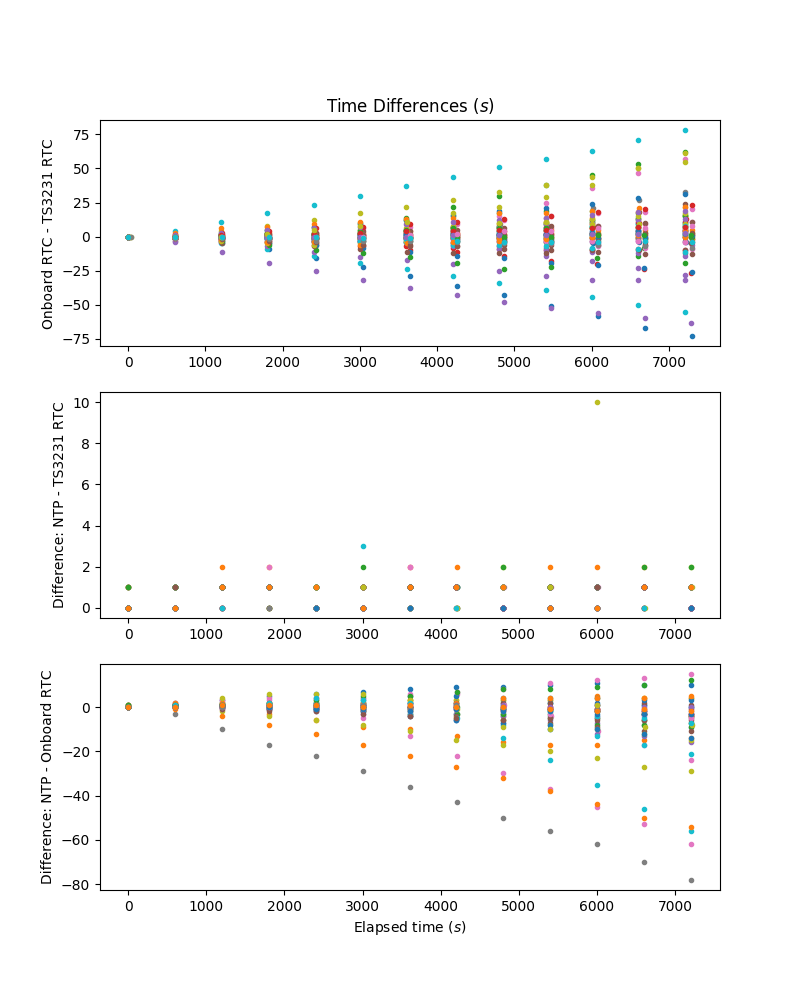
\includegraphics[width=\MFW]{/home/dg/PublicSensors/Textbooks/IntroSensors/Images/TimeAccPrecPlt1.png}}{https://publicsensors.org/IntroSensors/Images/TimeAccPrecPlt1.png}
			\caption[Plots of time-keeping errors]{Plots of time-keeping errors, indicated by differences among three methods of keeping time. 
			Top: Onboard \rtc minus \DS3231 \rtc. Middle: \ntp minus \DS3231 \rtc. Bottom: \ntp minus onboard \rtc. }
			\labfig{TAPplt1}
		\end{center}
	\end{marginfigure}
	
	When the scripts have run successfully, they will produce a set of plots like \reffig{TAPplt1}.
	\begin{itemize}
		\item[$\circ$] This example assumes the \lstinline{TimeData} subdirectory is in the same directory that contains \htmladdnormallink{TimeAccPrec.py}{https://publicsensors.org/IntroSensors/Codes/TimeAccPrec.py} and from which you launched the \python session.
		If you have used file names or directories other than these defaults, adjust your commands accordingly. 
		\item[$\circ$] The \lstinline{plt_style} parameter determines the type of symbol and line in the plots. 
		The value in the example, \lstinline{plt_style}, means that each data point will be plotted as a small circle, with no lines connecting sequential data points.
	\end{itemize}

	\item \textbf{Experiment with} \lstinline{matplotlib}\textbf{'s} \htmladdnormallink{interactive navigation widgets}{https://matplotlib.org/users/navigation_toolbar.html}:
	\begin{itemize}
		\item[$\circ$] The small buttons at the bottom left of the graphics window enable you to zoom and pan to different parts of your plots, and to save your figure as a \lstinline{png} or \lstinline{jpg} image.
		These images can be imported into a report or web page. 
		See the link above for detailed explanations of how these widgets work.  
		
		\smallskip
		When you are finished, close the figure window to be ready for the next steps in plotting data.
	\end{itemize}
%	\todo{milestone}
\loadMilestone{mlst:03a} % load milestone with tags id: mlst:02a

	\item \textbf{Replot time-keeping errors, using plotting symbols and line type to distinguish data from your own microcontroller/\rtc combination}:

	Repeat the commands you used to produce the previous plots, but instead of the previous call to \lstinline{lineplot_TC_data} substitute
\begin{lstlisting}[language=Python]
lineplot_TC_data(fig,axes,data_directory='TimeData',
        template="*.txt",plt_style='.',exclude='3648523')
lineplot_TC_data(fig,axes,data_directory='TimeData', 
        template="*3648523*.txt",plt_style='^:')
\end{lstlisting}
	where, as before, adjust as necessary to reflect your filenames and directories.
	\begin{marginfigure}[-19.cm]
		\begin{center}
			\htmladdnormallink{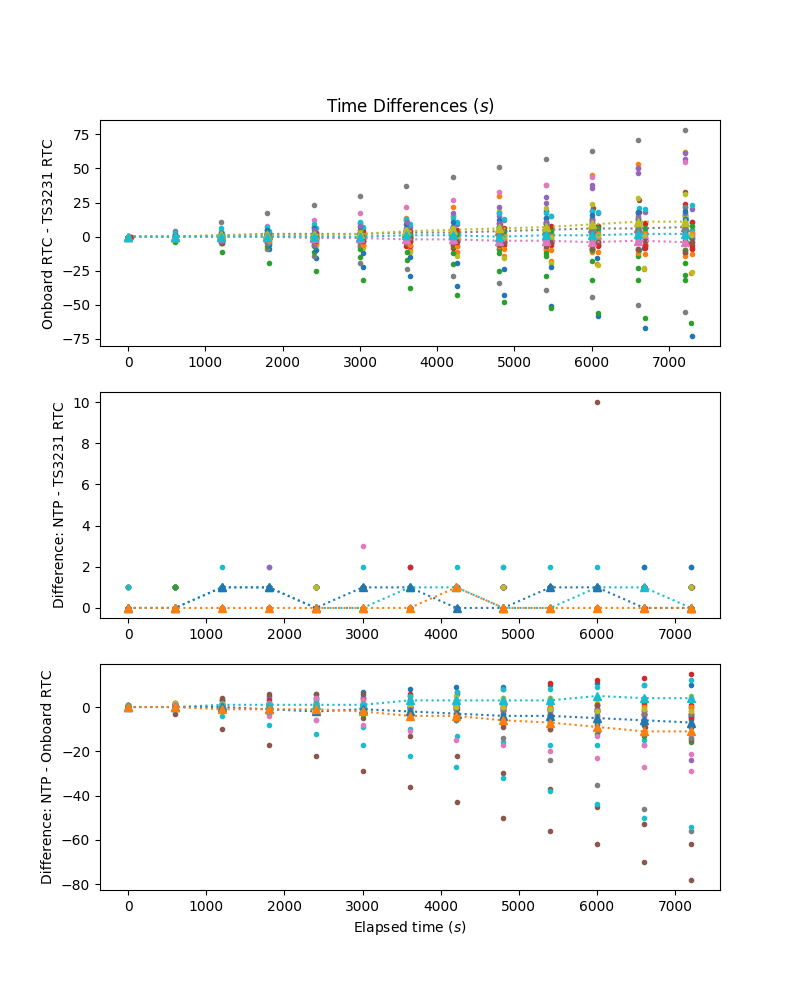
\includegraphics[width=\MFW]{/home/dg/PublicSensors/Textbooks/IntroSensors/Images/TimeAccPrecPlt2.png}}{https://publicsensors.org/IntroSensors/Images/TimeAccPrecPlt2.png}
			\caption[Plots of time-keeping errors]{Plots of time-keeping errors, indicated by differences among three methods of keeping time. 
			Triangles and dotted lines represent data from the focal microcontroller/\rtc combination. 
			Top: Onboard \rtc minus \DS3231 \rtc. Middle: \ntp minus \DS3231 \rtc. Bottom: \ntp minus onboard \rtc. }
			\labfig{TAPplt2}
		\end{center}
	\end{marginfigure}
	The resulting plot should look something like \reffig{TAPplt2}.
	\begin{itemize}
		\item[$\circ$] In the first of these commands, the parameter \lstinline{exclude='3648523'} means that any filename containing '3648523' will \underline{not} be plotted. 
		
		\smallskip
		'3648523' is the unique ROM ID of one of the microcontrollers used to collect the data archive. 
		Therefore, this command will plot all data 
		
		\item[$\circ$] In the second command, the parameter \lstinline{template="*3648523*.txt"} means that \underline{only} filenames containing '3648523' (and ending in `.txt') will be plotted. 
		
		\item[$\circ$] The parameter \lstinline{plt_style='^:'} means that data from filenames containing '3648523' will appear as triangles, connected by dotted lines.
		
		\item[$\circ$] Together, these commands results in plots showing data from microcontroller '3648523' as triangles connected by dotted lines, while all other data are plotted as unconnected circles.
		
		\smallskip
		Substitute your microcontroller's ROM ID into these commands to see how your microcontroller/\rtc combination compares to the overall population of 
		rtcs.
	\end{itemize}
%	\todo{milestone}
\loadMilestone{mlst:03b} % load milestone with tags id: mlst:02
	
	\item \textbf{Use the \python method \lstinline{subsample_TC_data} to collect a subsample of the time-keeping error data}:
	
	Use a command like:
\begin{lstlisting}[language=Python]
(subsample_times,subsample_onbrd_ext,subsample_NTP_ext,subsample_NTP_onbrd)= \
subsample_TC_data(data_directory='TimeData', template="*.txt",sub_samples=[0,3,6,9,12],exclude='3648523')
\end{lstlisting}
	where as before you have adjusted the filenames and directory as necessary.

	In this command, the parameter \lstinline{sub_samples=[0,3,6,9,12]} means data will be retained only from sample numbers 0,3,6,9,and 12 (in this case, at half hour intervals because samples are ten minutes apart). 

	The ``subsample'' lists on the left side contain the elapsed time and error data from the selected sample numbers.
	
	\item \textbf{Replot the time-keeping plots, adding percentiles to inform you how your microcontroller/\rtc combination compares to the population of \rtcs}:
	To make this plot, repeating all the previous steps you used to create a figure window, parse and plot data, \etc, but before you ``show'' the plot execute the command
\begin{lstlisting}[language=Python]
prcntplot_TC_data(fig,axes,subsample_times,subsample_onbrd_ext,
      subsample_NTP_ext,subsample_NTP_onbrd,pcnts=[5.,25.,50.,75.,95.])
\end{lstlisting}
	This command uses the subsampled data to generate plots with lines for specified percentiles.
	In this case, the parameter \lstinline{pcnts=[5.,25.,50.,75.,95.]} specifies that the 5th, 25th, 50th, 75th and 95th percentiles are to be plotted.
	\begin{marginfigure}[-19.cm]
	\begin{center}
		\htmladdnormallink{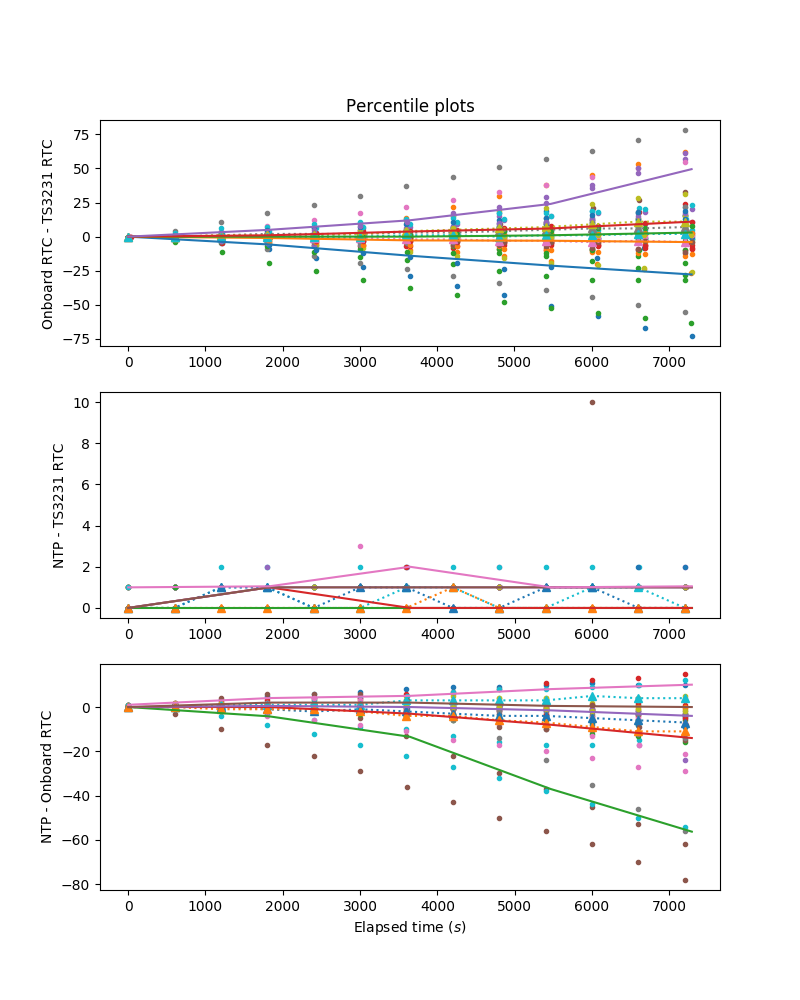
\includegraphics[width=\MFW]{/home/dg/PublicSensors/Textbooks/IntroSensors/Images/TimeAccPrecPlt3.png}}{https://publicsensors.org/IntroSensors/Images/TimeAccPrecPlt3.png}
		\caption[Plots of time-keeping errors]{Plots of time-keeping errors, indicated by differences among three methods of keeping time. 
		Triangles and dotted lines represent data from the focal microcontroller/\rtc combination. 
		Solid lines represent selected percentiles (5th, 25th, 50th, 75th and 95th), excluding data from the focal microcontroller/\rtc combination. 
		Top: Onboard \rtc minus \DS3231 \rtc. Middle: \ntp minus \DS3231 \rtc. Bottom: \ntp minus onboard \rtc. }
		\labfig{TAPplt3}
	\end{center}
\end{marginfigure}

	\smallskip
	The resulting plot --- something like \reffig{TAPplt3} --- enables you to see at a glance how the time-keeping errors from your microcontroller/\rtc combination compare to various percentiles of errors from the population of devices.
%	\todo{milestone}
\loadMilestone{mlst:03c} % load milestone with tags id: mlst:02
	
	\item \textbf{Generate violin plots to visualize the distributions of time-keeping errors in the subsampled data}:
\begin{lstlisting}[language=Python]
violinplot_TC_data(fig,axes,subsample_times,subsample_onbrd_ext,subsample_NTP_ext,subsample_NTP_onbrd,v_widths=200.,bw=0.5)
\end{lstlisting}
	\begin{marginfigure}[0.cm]
	\begin{center}
		\htmladdnormallink{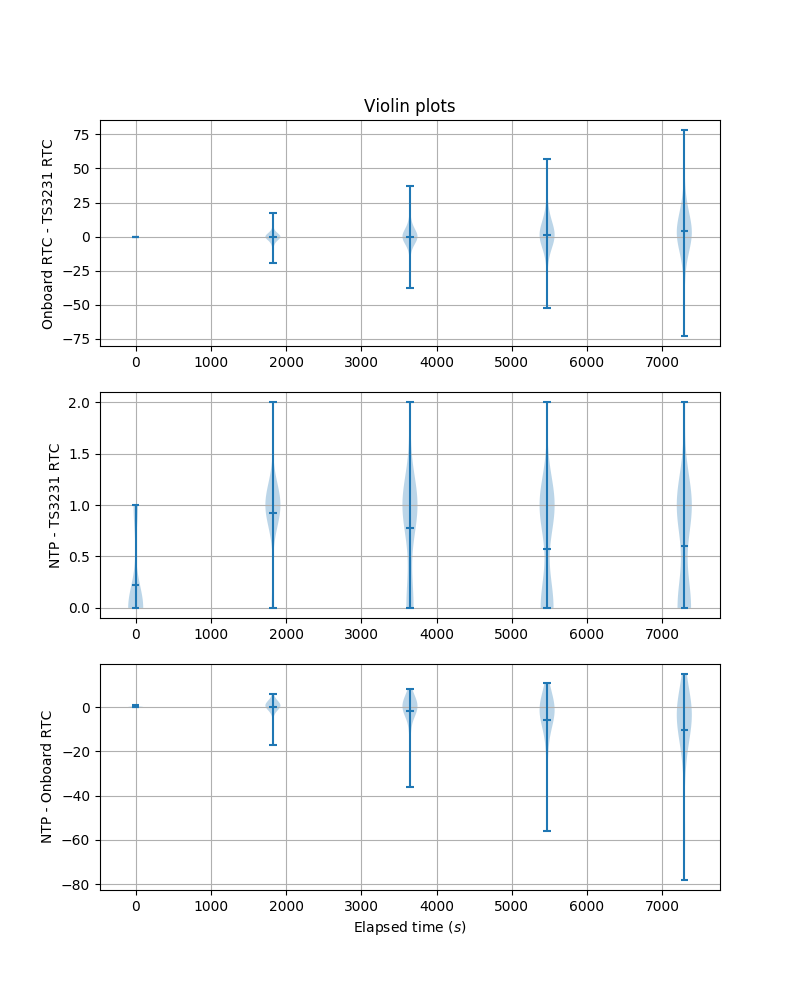
\includegraphics[width=\MFW]{/home/dg/PublicSensors/Textbooks/IntroSensors/Images/TimeAccPrecPlt4.png}}{https://publicsensors.org/IntroSensors/Images/TimeAccPrecPlt4.png}
		\caption[Violin plots of time-keeping errors]{Violin plots of time-keeping errors, indicated by differences among three methods of keeping time.
		Top: Onboard \rtc minus \DS3231 \rtc. Middle: \ntp minus \DS3231 \rtc. Bottom: \ntp minus onboard \rtc. }
		\labfig{TAPplt4}
	\end{center}
\end{marginfigure}
	This command results in plots like \reffig{TAPplt4}.
	You can vary the parameters \lstinline{v_widths=200.,bw=0.5} to adjust the width and breadth of the resulting distributions to get a good representation of your data.
	Details about implementation of violin plots are given in \lstinline{matplotlib}'s \htmladdnormallink{documentation}{	https://matplotlib.org/3.1.1/api/_as_gen/matplotlib.pyplot.violinplot.html}.
	
	Note the differences in vertical axes. 
	What can you say about the distributions of time-keeping errors?
	Are they \texttt{unimodal} or \texttt{multi-modal}?
	Do they reflect directional biases towards being more often negative than positive, or \textit{vice versa}?
	What can you say, based on the plots you've generated, about the relative magnitudes of errors for the different time-keeping methods?
%	\todo{milestone}
\loadMilestone{mlst:03d} % load milestone with tags id: mlst:02
	
\end{enumerate}

\subsection{Hypothesis tests about \rtc accuracy and precision}
We now turn to \emph{hypothesis tests} about errors associated with the different methods of keeping time with microcontrollers. 
Recall that hypothesis tests quantify the probability an observed outcome occurred by chance, if some assumptions about the statistical distributions are true.
The tests are usually posed in the form of a \emph{null hypothesis}, e.g. that two datasets are drawn from the same distribution. 

Statistical analysis enables us to calculate the probability with which the observed results could have happened, assuming the assumptions and null hypothesis are true. 
The lower the resulting probability, the less likely it is that the null hypothesis is true.
If the probability is less than a threshold --- usually $0.05$, or 1 in 20 --- we consider it so unlikely that we accept the null hypothesis is \emph{falsified}.
Falsifying the hypothesis that two distributions are the same implies that the distributions are significantly different.

Note that the converse does not apply. 
If the resulting probability is above the threshold, that does not prove the distributions are the same --- only that we failed to establish that they are different.
It may be that they are truly the same, but it may also be that they are different and our statistical sampling was insufficient to demonstrate it.

For example, consider the question ``Is my \rtc defective?'' 
In statistical terms, this question can be made more explicit by restating it as ``Are the time-keeping errors from my \rtc different than the errors from the whole population of \rtcs?''
This statistical form of the question can be tested in the form of a null hypothesis: 
\begin{itemize}
	\item[$\circ$]The distribution of errors from my \rtc is the same as the distribution of errors from the  whole population of \rtcs.
\end{itemize}
Because you have time-keeping error samples from your \rtc and a population of other \rtcs, you can estimate the probability that your samples could have been drawn from the whole population of \rtcs.
This probability can be estimated in several ways, depending on what we know about the characteristics of the distributions. 

If we know nothing about the observed error distributions, or if we know their shapes but they does not conform to any standard distribution, we can use \emph{non-parametric tests}.
Non-parametric tests rely only on the order of samples in two datasets, not the shape of their distributions.
Among the most useful non-parametric tests are:
\begin{itemize}
	\item[$\circ$] The \emph{Wilcoxon rank-sum test}, which tests the \htmladdnormallink{null hypothesis that two sets of samples are drawn from the same distribution}{https://docs.scipy.org/doc/scipy/reference/generated/scipy.stats.ranksums.html\#scipy.stats.ranksums}. 
	\item[$\circ$] The \emph{Kruskal-Wallis H-test}, which tests the  \htmladdnormallink{null hypothesis that the medians of two datasets are the same}{https://docs.scipy.org/doc/scipy/reference/generated/scipy.stats.kruskal.html\#scipy.stats.kruskal}.
\end{itemize}
Applied to your datasets, if either or both of these null hypotheses can be falsified, the implication is that your \rtc is defective.
If neither can be falsified, that implies a lack of evidence that your \rtc is defective. 
That is, the combination of the data and non-parametric tests lack the \emph{power} to establish a significant difference.
The possibility remains that with much larger sample size, or longer sampling time, the hypotheses could be falsified. 
Or, your \rtc might really not be defective!

If we knew that time-keeping errors conform to a standard distribution, we might be able to use more discriminating hypothesis tests.
For example, if we knew that these errors are normally distributed, we could use
\begin{itemize}
	\item[$\circ$] The \emph{T-test}, which tests the  \htmladdnormallink{null hypothesis that the means of two sets of normally distributed data are the same}{https://docs.scipy.org/doc/scipy/reference/generated/scipy.stats.ttest_ind.html\#scipy.stats.ttest_ind}.
\end{itemize}
The \emph{T-test} null hypothesis is similar to the \emph{Kruskal-Wallis H-test}, but focuses on the mean rather than the median.
The requirement that both datasets have normal (a.k.a. \emph{Gaussian}) distributions means that the plausible range of means can be better constrained.
Compared to the non-parametric tests, this tighter constraint makes the \emph{T-test} more powerful for a given set of data. 
A \emph{T-test} can potentially falsify the null hypothesis even when the corresponding \emph{Kruskal-Wallis H-test} can not.

\subsubsection{\howto Probability plots and hypothesis tests with \rtc data}
\begin{enumerate}
	\item \textbf{If they are not already imported, import the required \python libraries}:
\begin{lstlisting}[language=Python]
import matplotlib.pyplot as plt
import scipy.stats as stats
from TimeAccPrec import * 
\end{lstlisting}
	\item \textbf{Separately sub-sample the data from your \rtc and from all the other \rtcs, with a modification of}:
\begin{lstlisting}[language=Python]
(subsample_times,subsample_onbrd_ext,subsample_NTP_ext,subsample_NTP_onbrd)= \
     subsample_TC_data(data_directory='TimeData', template="*.txt",sub_samples=[0,3,6,9,12],exclude='3648523')
(subsample_times2,subsample_onbrd_ext2,subsample_NTP_ext2,subsample_NTP_onbrd2)= \
     subsample_TC_data(data_directory='TimeData', template="*3648523*.txt",sub_samples=[0,3,6,9,12])
\end{lstlisting}
	\item \textbf{Graphically assess whether the error distributions conform to a normal distribution}:
\begin{lstlisting}[language=Python]
fig,axes=plt.subplots(nrows=3,ncols=1,figsize=(8,10))
dstr=stats.norm
probplot_TC_data(axes[0],subsample_onbrd_ext,'onbrd_ext',dst=dstr)
probplot_TC_data(axes[1],subsample_NTP_ext,'NTP_ext',dst=dstr)
probplot_TC_data(axes[2],subsample_NTP_onbrd,'NTP_onbrd',dst=dstr)
# Add a title and "show" the plots:
axes[0].set_title('Probability plots')
plt.show()
\end{lstlisting}
	\begin{marginfigure}[-19.cm]
	\begin{center}
		\htmladdnormallink{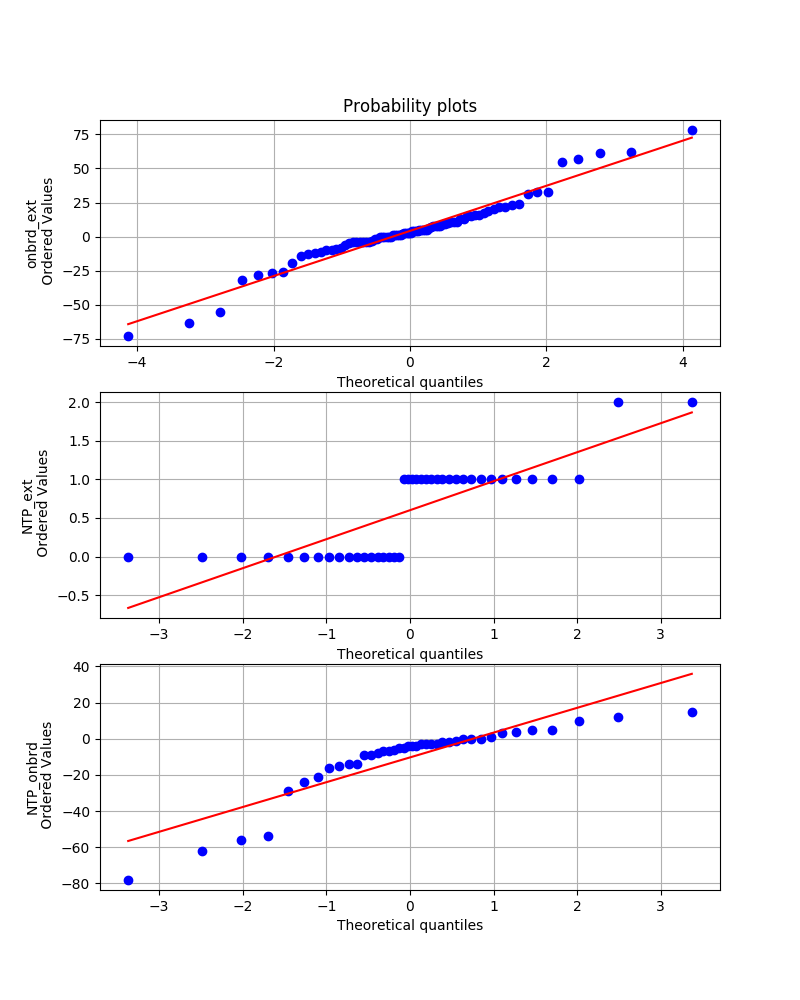
\includegraphics[width=\MFW]{/home/dg/PublicSensors/Textbooks/IntroSensors/Images/TimeAccPrecPlt5.png}}{https://publicsensors.org/IntroSensors/Images/TimeAccPrecPlt5.png}
		\caption[Probability plots of time-keeping errors]{Probability plots of time-keeping errors assuming a normal distribution, indicated by differences among three methods of keeping time.
			Top: Onboard \rtc minus \DS3231 \rtc. Middle: \ntp minus \DS3231 \rtc. Bottom: \ntp minus onboard \rtc. }
		\labfig{TAPplt5}
	\end{center}
\end{marginfigure}
	The result of these commands, similar to \reffig{TAPplt5}, indicate which differences among time-keeping methods conform to a normal distribution.
	The closer the plotted data points lie to the red line, the more normally distributed they are.
	
	\smallskip
	Note that \lstinline{probplot_TC_data} plots only the last sampling interval in the subsampled dataset. 
	
	\smallskip
	\texttt{scipy}'s plotting algorithm also provides some useful quantitative metrics:
	\begin{itemize}
		\item[$\circ$] The \texttt{intercept} of the regression (red) line indicates the mean of the approximating normal distribution.
		\item[$\circ$] The \texttt{slope} of the regression (red) line indicates the variance of the approximating normal distribution.
		\item[$\circ$] The square root of the \texttt{Coefficient of Determination} indicates goodness of fit between the data and the approximating normal distribution.
	\end{itemize}
	
	
	In \reffig{TAPplt5}, the differences in the archived dataset between the onboard and external \rtcs (top plot) are reasonably close to normally distributed.
	There are noticeable deviations at the left and right sides (corresponding to the tails of the distributions). 
	The other error distributions appear less consistent with a normal distribution.
\loadMilestone{mlst:03e} % load milestone with tags id: mlst:02

	\item \textbf{Perform hypothesis tests comparing your \rtc to the whole population of \rtcs}:
\begin{lstlisting}[language=Python]
hypothesis_TC_data(subsample_times,subsample_onbrd_ext,subsample_onbrd_ext2,pcnts=[5.,25.,50.,75.,95.])
\end{lstlisting}
	In this example, we have focused on the time-keeping differences between the onboard and external \rtcs,but in working with your data you can make other comparisons.

	\smallskip
	The output of this command has two parts:
	\begin{itemize}
		\item[$\circ$] The first part of the output summarizes the distributions by printing out their percentiles at each of the sub-sampling intervals.
		\item[$\circ$] The second part prints out the results of three hypothesis tests (Kruskal-Wallis H-test, Wilcoxon rank-sum and T-test) at each of the sub-sampling intervals.
		
		\smallskip
		The key output is the $p$-value, representing the probability of getting the observed data if the null hypothesis is true.
		
		\smallskip
		Note that the T-test analysis gives a result, but that result has statistical validity only if the underlying assumption that time-keeping errors are normally distributed are satisfied.
	\end{itemize}

\end{enumerate}
\loadMilestone{mlst:03f} % load milestone with tags id: mlst:02


\subsection{Environmental effects on \rtc accuracy and precision}
At this point, you have developed the skills to build a dataset of time-keeping errors, using differences among the three methods of time-keeping. 
You have experience in a variety of plotting techniques, that enable you to visualize the overall distribution of time-keeping errors, the percentiles of devices that show specific magnitudes and directions of errors, and how a sub-sample of devices compare to the entire population. 
You have also applied hypothesis testing techniques, with consideration of which statistical tests are applicable to the error distributions in your dataset.
This work has given you a basis for anticipating which time-keeping methods are most accurate and precise, how large errors are likely to be, and whether a given device appears to be more error-prone than expected.

It's worth considering how these results apply to the sensors you will deploy in the field. 
Field conditions for environmental sensors vary widely, including wide ranges in temperature, humidity, salinity, incident solar radiation, pressure, and other environmental parameters. 
Because your microcontroller/\rtc combination will be within an environmental housing, it will not be exposed to many of these variations. 
However, environmental housings do not typically insulate devices from temperature fluctuations.
In fact, the internal temperatures inside housings often range over much wider extremes than the ambient environment.
For example, temperature inside an environmental housing exposed to direct sunshine can reach 10s of degrees higher than the surrounding air. 
Conversely, internal temperature can reach well below freezing.

Temperature has strong effects on many electrical and mechanical material properties. 
For this reason, devices with \rtcs have built-in thermometers, and algorithms to compensate for temperature effects on vibrating crystals and other components.
There is clearly the possibility that these thermometers and algorithms involve substantial additional errors.
If so, the performance of our time-keeping devices might be very different in the field than in our laboratory tests.

In generating and analyzing the time-keeping datasets, we have not paid particular attention to environmental conditions. 
During data collection, the microcontrollers and \rtcs were likely under relatively comparable conditions, e.g. in the same laboratory, or under similar but haphazardly varying conditions (e.g. room temperatures in different classmates' houses).
By repeating your data collection and analysis, but with an experimental design that explicitly designates two subpopulations operating at different temperatures, you can quantify the effects (if any) of temperature on the error distributions of time-keeping devices.

\subsubsection{\howto Quantifying temperature effects on time-keeping errors}
Use the methods of this chapter in collaboration with your classmates to test the null hypothesis that:
\begin{itemize}
	\item[$\circ$] Time-keeping errors from microcontroller/\rtc combinations operated at environmentally relevant low and high temperatures have the same statistical distributions.
\end{itemize}
\begin{enumerate}
	\item \textbf{Agree on a consensus sampling protocol, with subpopulations divided into ``hot'' and ``cold'' subpopulations.}
	
	In designing your protocol, consider the trade-offs between longer sample duration \textit{vs} more replicates, within a practical total available time for data collection.
	In choosing ``hot'' and ``cold'' temperatures for this experiment, it's likely that you will need to make concessions to practical constraints.
	In many cases, using outdoor conditions for the hot or cold subpopulations might be practical.
	Make sure, however, that your devices are protected from moisture and other damaging conditions, e.g. by placing them in a sealed plastic bag. 
	
	\item \textbf{Visualize the resulting populations, using different plotting symbols and line types to indicate how percentiles evolve over time and assess distribution shapes.}
	\item \textbf{Perform statistical tests of the null hypothesis, using the non-parametric tests and --- if justified --- the \texttt{T-test}.}
	
	
\end{enumerate}

\loadMilestone{mlst:03g} % load milestone with tags id: mlst:02


%This provides a basis for 
%
%DEFINE HYPOTHESES TO START WITH:
%-- ONE RTC IS DIFFERENT FROM OTHERS
%-- ERRORS DUE TO METHOD X ARE WITHIN BOUNDS Y
%-- ERRORS ARE A FUNCTION OF ENVIRONMENT E.G. TEMPERATURE
%
%will assess the relative \emph{accuracy} and \emph{precision} of each method. 
%Refer to the \refsec{acc_prec} if you want a reminder of the distinctions between accuracy and precision.
%



%of observed timekeeping errors (). 
%(A) Data parsing and visualization (1.5 points) 
%In this section of the problem set, you will use a python script to parse and plot our dataset. The script is called \lstinline{analyze_acc_prec_OCN351.py}, and it is posted in Files>MicroPython on Canvas. 
%
%Download \lstinline{analyze_acc_prec_OCN351.py}, and place it in your python code folder.
%
%The dataset is also posted in the MicroPython directory, in a zipped archive called PS1timedates.zip. Download and unzip this file into a directory on your computer.
%
%Modify the code to make it work on your machine. This step may take some trial and error – please contact the instructors if you have persistent trouble with any of the necessary adjustments.
%
%One change you will need to make is to edit the string \lstinline{data_directory} (line 14), so that it points to the folder in which you placed the PS1timedates data directory. Keep in mind that, in Linux OS, the separator between different levels in the file structure is a ``/''. It is the same on MacOS, but different on Windows. 
%
%When this python code executes, it reports the names of the data files it has found and the number of lines it parsed from each. This makes it easy to tell whether the directory information is correct.
%
%When execution is complete, you should see a graphics window with 6 plots. In each row, the left column is a plot of the observed differences between two time sources. The right plot is a violin plot, in which the blue shading represents an estimate of the distribution of differences at specific time points (determined by sample numbers in violin\textunderscore sample). Error levels where the shading is wide are relatively more frequent in the data than levels where the shading is narrow.
%
%
% After making adjustments so that your code finds the data and produces plots, spend a few minutes experimenting with settings and parameters to see what they do. 
%
%The width and degree of smoothing in the violin plots are determined by the parameters v\textunderscore widths and bw. Do some settings appear more informative about timekeeping errors than the default ones?
%
%Save the figure(s) you produce by clicking the rightmost icon on the bottom bar.



	
%How can we quantify time-keeping errors? 
%
%To begin with, we need some way to determine ``true'' time, from a reference time source that we believe to have time-keeping errors that are so small as to be negligible for our purposes. 
%An example is the \htmladdnormallink{official time source}{https://www.time.gov/} for the U.S. government, operated by the National Institute of Standards and Technology (NIST).
%
%Assuming we have an accurate reference, let's suppose we use a device to take a large number --- hundreds or even thousands --- of time measurements, over a specific ``true'' time interval, such as an hour. 
%
%How do we know what ``true'' time? We need to use a reference time source, 


%We will collect timestamp data from each of your microcontrollers to answer the following questions:
%\begin{itemize}
%	\item How accurate and precise are each of the methods of obtaining the current time?
%	\item Do the RTCs on different microcontrollers differ \emph{systematically} from each other (that is, are particular \rtcs biased towards run fast or slow)?
%	\item Does the magnitude and direction of timekeeping error depend on environmental conditions (e.g. temperature)?  
%\end{itemize}


